\documentclass{article}
\usepackage{lipsum}
\usepackage{authblk}
\usepackage{listings}
\usepackage{xcolor}
\usepackage{hyperref}
\usepackage{tikz}
\usetikzlibrary{shapes.geometric, arrows}
\usepackage[utf8]{inputenc}
\usepackage{subcaption}
\usepackage{caption}
\usepackage{amssymb}
\usepackage{amsmath}
\usepackage[hidelinks]{hyperref}
\usepackage[svgnames]{xcolor}
\usepackage[a4paper,total={7in, 8in}]{geometry}
\usepackage{bm}
\usepackage{centernot}
\usepackage{titling}
\usepackage{color}
\usepackage{listings}
\usepackage{listings-rust}
\usepackage{graphicx} % Required for inserting images
\usepackage{tikz}
\tikzstyle{mybox} = [draw=black, thin, rectangle, rounded corners, inner ysep=5pt, inner xsep=5pt, fill=orange!20]


%Per disegnare il box
%\hspace*{-5mm}
%\begin{tikzpicture}
%\node [mybox] (box){%
%    \begin{minipage}{.96\textwidth}     %Larghezza del box
            %Qui testo
%    \end{minipage}
%};
%\end{tikzpicture}%



% Stili per i nodi e le frecce
\tikzstyle{block} = [rectangle, minimum width=2.5cm, minimum height=1cm, text centered, draw=black]
\tikzstyle{run1} = [block, fill=orange!40]
\tikzstyle{run2} = [block, fill=blue!40]
\tikzstyle{run3} = [block, fill=purple!40]
\tikzstyle{arrow} = [thick,->,>=stealth]

\title{\textbf{[Manuale Utente] Realizzazione di un ambiente di fault injection per applicazione ridondata}}

\author{Carlo Migliaccio}
\author{Federico Pretini}
\author{Alessandro Scavone}
\author{Mattia Viglino}
\affil[1]{\small{Laurea Magistrale in Ingegneria Informatica, Politecnico di Torino}}

\date{Gennaio 2025}

\pagestyle{headings}

\begin{document}

\counterwithin{figure}{section}
\counterwithin{equation}{section}
\renewcommand{\labelenumii}{\arabic{enumi}.\arabic{enumii}}

\maketitle
\thispagestyle{empty}
\vspace{-0.8cm}
\tableofcontents

\section*{Introduzione}
Questo manuale fornisce istruzioni rapide per utilizzare il programma scritto in Rust. Il programma consente di navigare attraverso un menu interattivo per eseguire varie operazioni.

\section*{Requisiti}
\begin{itemize}
\item \textbf{Sistema operativo}: macOS, Linux o Windows.
\item \textbf{Compilatore Rust}: \texttt{rustc} installato. Puoi installarlo da \url{https://rustup.rs}.
\end{itemize}

\section*{Come Aprire ed Eseguire il Programma}
\begin{enumerate}
\item Accedere alla directory che contiene il file \texttt{Cargo.toml} del progetto.
\item Eseguire il programma tramite un tool grafico o con il comando \texttt{cargo run}.
\end{enumerate}

\section*{Guida al Menu}
Dopo l'avvio, il programma presenterà un menu interattivo. La scelta corrente è evidenziata da un indicatore visivo (\texttt{>}), che consente all'utente di identificare chiaramente l'opzione selezionata. \\ 
Per navigare tra le opzioni del menu, utilizza i tasti freccia \texttt{Su} e \texttt{Giù}.\\
Premendo il tasto \texttt{Invio}, confermerai la tua selezione. \\ 
Quando viene proposta una selezione predefinita, questa è racchiusa tra parentesi quadre. Puoi accettarla semplicemente premendo \texttt{Invio}.

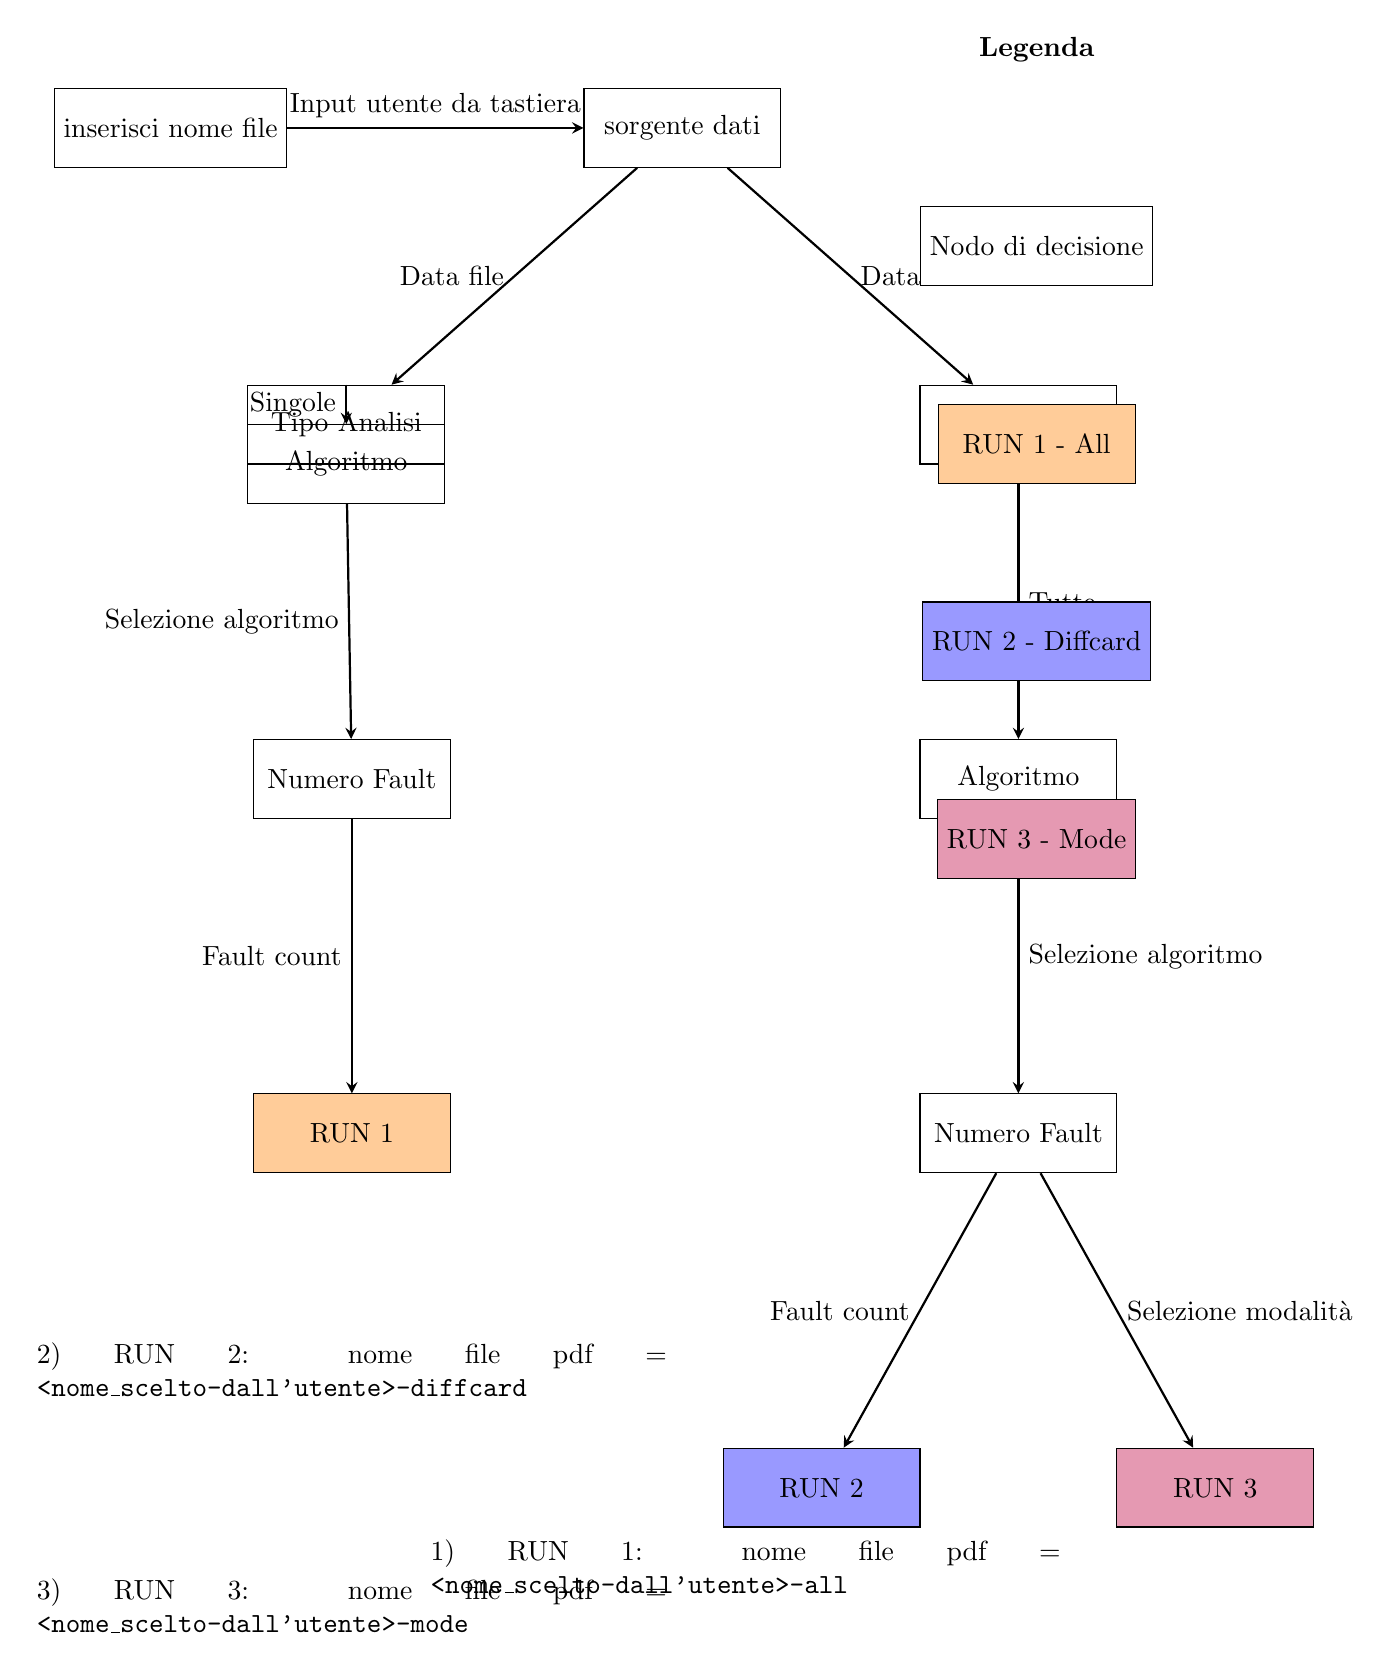
\begin{tikzpicture}[node distance=2.5cm]
% Nodi principali
\node (fileinput) [block] {inserisci nome file};
\node (datasource) [block, right of=fileinput, xshift=4cm] {sorgente dati};
\node (analysis1) [block, below left of=datasource, yshift=-2cm, xshift=-2.5cm] {Tipo Analisi};
\node (analysis2) [block, below right of=datasource, yshift=-2cm, xshift=2.5cm] {Tipo Analisi};
\node (algorithm1) [block, below of=analysis1, yshift=+2cm] {Algoritmo};
\node (algorithm2) [block, below of=analysis2, yshift=-2cm] {Algoritmo};
\node (numfault1) [block, below of=analysis1, yshift=-2cm, xshift=2] {Numero Fault};
\node (numfault2) [block, below of=algorithm2, yshift=-2cm] {Numero Fault};
\node (run1) [run1, below of=numfault1, yshift=-2cm] {RUN 1};
\node (run2) [run2, below of=numfault2, yshift=-2cm, xshift=-2.5cm] {RUN 2};
\node (run3) [run3, below of=numfault2, yshift=-2cm, xshift=2.5cm] {RUN 3};

% Frecce e testi sulle connessioni
\draw [arrow] (fileinput) -- (datasource) node[midway, above] {Input utente da tastiera};
\draw [arrow] (datasource) -- (analysis1) node[midway, left] {Data file};
\draw [arrow] (datasource) -- (analysis2) node[midway, right] {Dataset};
\draw [arrow] (analysis1) -- (algorithm1) node[midway, left] {Singole};
\draw [arrow] (analysis2) -- (algorithm2) node[midway, right] {Tutte};
\draw [arrow] (algorithm1) -- (numfault1) node[midway, left] {Selezione algoritmo};
\draw [arrow] (algorithm2) -- (numfault2) node[midway, right] {Selezione algoritmo};
\draw [arrow] (numfault1) -- (run1) node[midway, left] {Fault count};
\draw [arrow] (numfault2) -- (run2) node[midway, left] {Fault count};
\draw [arrow] (numfault2) -- (run3) node[midway, right] {Selezione modalità};

% Legenda
\node (legendtitle) [right of=datasource, xshift=2cm, yshift=1cm, text width=4cm, text centered] {\textbf{Legenda}};
\node (legendinput) [block, below of=legendtitle, fill=white] {Nodo di decisione};
\node (legendrun1) [run1, below of=legendinput, yshift=-0.01cm] {RUN 1 - All};
\node (legendrun2) [run2, below of=legendrun1, yshift=-0.01cm] {RUN 2 - Diffcard};
\node (legendrun3) [run3, below of=legendrun2, yshift=-0.01cm] {RUN 3 - Mode};

% Note finali
\node (note1) [below of=run1, xshift=5cm, yshift=-3cm, text width=8cm, text justified] {1) RUN 1: nome file pdf = \texttt{<nome\_scelto-dall'utente>-all}};
\node (note2) [below of=run1, yshift=-0.5cm, text width=8cm, text justified] {2) RUN 2: nome file pdf = \texttt{<nome\_scelto-dall'utente>-diffcard}};
\node (note3) [below of=note2, yshift=-0.5cm, text width=8cm, text justified] {3) RUN 3: nome file pdf = \texttt{<nome\_scelto-dall'utente>-mode}};
\end{tikzpicture}

\end{document}
